%*************************************************************************************************************************
\section{Uncertainty Quantification in Nuclear Engineering Thermal-Hydraulics}\label{sec:intro_uncertainty_quantification}
%*************************************************************************************************************************

% Introductory Paragraph
Before continuing the discussion of uncertainty analysis of code predictions, it will be worthwhile to define some additional terminologies to avoid later confusion.

In making a connection with the notion of simulator \emph{simulator} introduced in Section~\ref{sec:intro_computer_simulation}, 
recall that from Fig.~\ref{fig:ch1_th_system_code} an \emph{input deck} is distinct from the code itself.
Fig.~\ref{fig:ch1_simulator_io} depicts the notion of simulator of a thermal-hydraulics system in a more generic way, as an input/output model.
\begin{figure}[bth]	
	\centering
	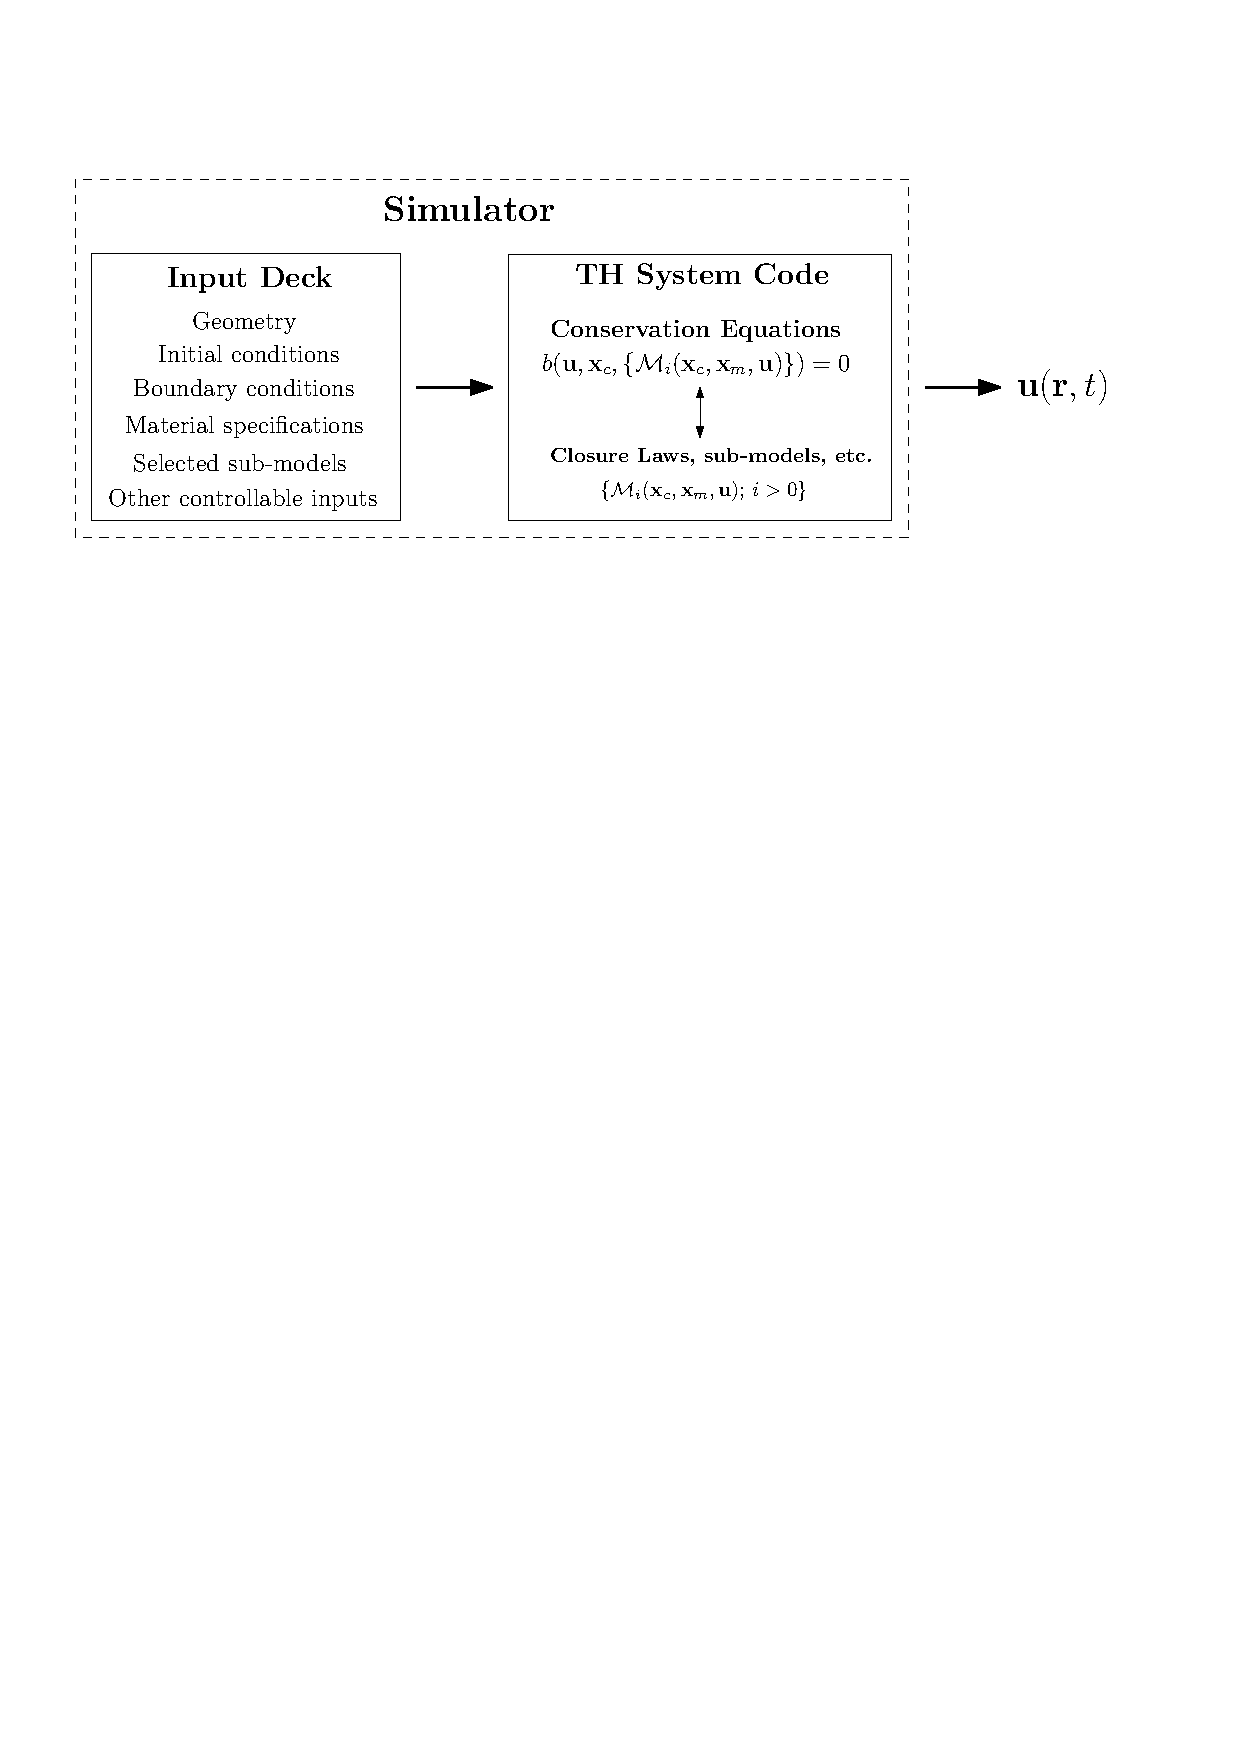
\includegraphics[width=\textwidth]{../figures/chapter1/figures/simulator_io}
	\caption[Simplified illustration of a simulator as an input/output model.]{Simplified illustration of a simulator as an input/output model.}
	\label{fig:ch1_simulator_io}
\end{figure}

Indeed input deck defines specific problem (i.e., system) of interest.
It includes the specifications for geometrical configuration (i.e., the nodalization), choice of material and fluid involves, as well as initial and boundary conditions.
It may also include the setting for the numerical solver.
Some of those specifications (such as the boundary conditions, etc.) are parametrized and constitutes \emph{controllable inputs} denoted by $\bm{x}_c$.
The conservation equations of the code are closed with additional set of closure laws (and other sub-models) $\mathcal{M}_i(\bm{x}_c, \bm{x}_m, \bm{u})$.
These closure laws are, in turn, parametrized with a set of model specific parameters denoted by $\bm{x}_m$ which is referred to as the \emph{physical model parameters}.
 
Specifying the input deck, as far as user is concerned, completely defines the problem and the code will solve the conservation equations which output the dynamic state of relevant physical variables $\mathbf{u}(\bm{r}, t)$ (e.g., fluid pressure, temperature, wall temperature, etc.).
In practice, these raw simulation outputs are further post-processed to obtain the so-called \glspl[hyper=false]{qoi} the are relevant to the problem at hand.

%--------------------------------------------------------------------------
\subsection{Forward Uncertainty Quantification}\label{sub:intro_uq_forward}
%--------------------------------------------------------------------------

% Best-estimate, limitation
As explained, best-estimate analysis uses more realistic modeling assumptions for analyzing transient behavior of \gls[hyper=false]{npp}.
It attempts as realistically as possible to describe the behavior of the relevant physical processes occur during the plant transient.
And yet, even the best available understanding of the physical process is still limited.
Understanding of complex phenomena might not yet adequate and data support for some processes can be very limited.
Simplifying assumptions, approximations, and expert judgments to some degree are unavoidable and still required to have a complete analysis.

% Best-estimate, plus uncertainty
Hence, best-estimate analysis has to be complemented with uncertainty analysis.
The ultimate goal of uncertainty analysis is to associate code prediction with its uncertainty.
These combined quantities are then compared with certain regulator safety limits (e.g., \gls[hyper=false]{pct}) to check whether the limits still fall outside the uncertainty band of the code prediction.

% Source of possible uncertainties

% Statistical uncertainty analysis, Inputs as random variables 

% Source of uncertainty, initial and boundary condition

% Source of uncertainty, physical model parameters
\begin{figure}[bth]	
	\centering
	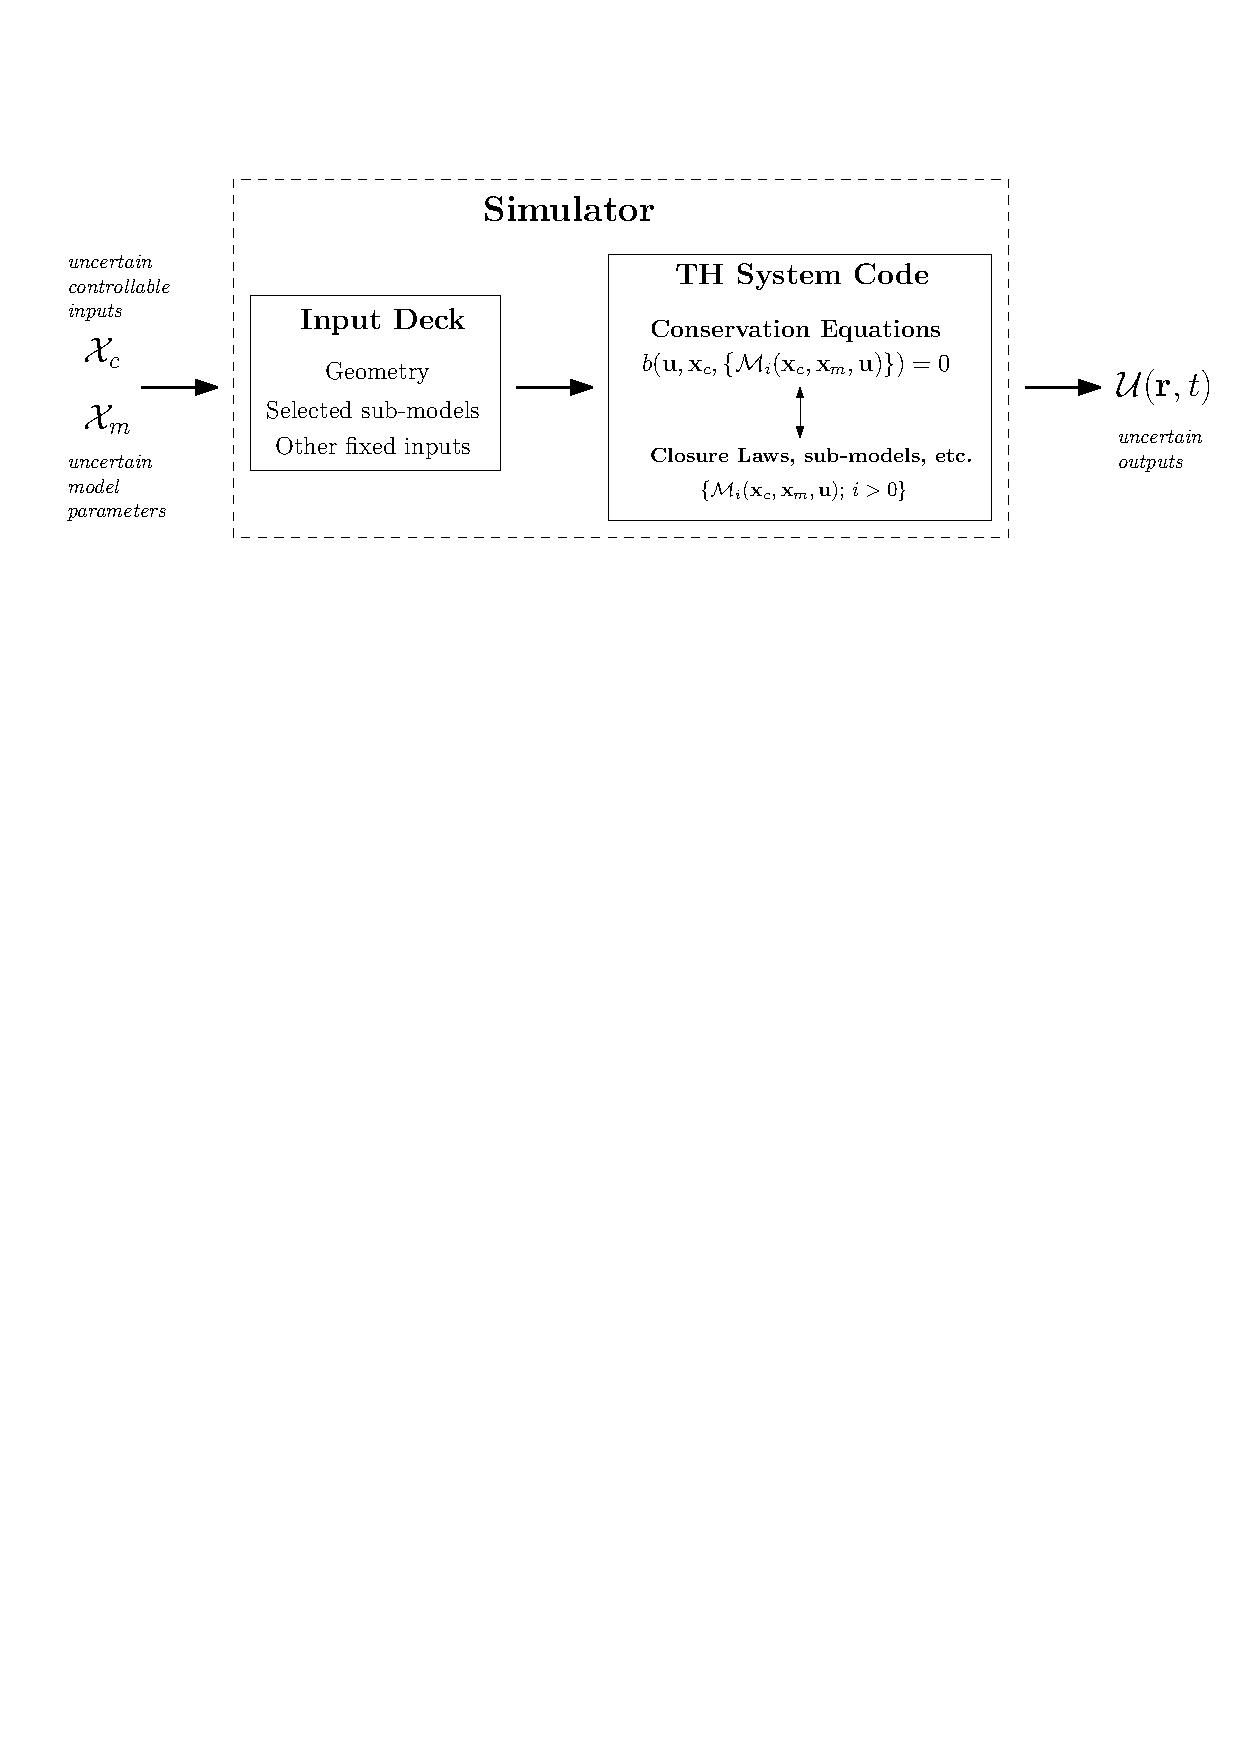
\includegraphics[width=\textwidth]{../figures/chapter1/figures/simulator_uq_forward}
	\caption[Simplified flowchart of forward uncertainty quantification of a simulator prediction.]{Simplified flowchart of forward uncertainty quantification of a simulator prediction.}
	\label{fig:ch1_simulator_uq_forward}
\end{figure}

%--------------------------------------------------------------------------
\subsection{Inverse Uncertainty Quantification}\label{sub:intro_uq_inverse}
%--------------------------------------------------------------------------

% Introductory paragraph, motivation
The physical model parameters often cannot be measured directly.
To estimate their values, basic experiments of well-specified conditions are carried out and correlations are fitted based on the experimental data. 
Recall that from the discussion of closure laws origin in Section~\ref{sub:intro_th_system_code},
this can also apply to phenomenological models where free parameters are allowed to be tuned according to match the experimental data.
Ultimately, the optimal value of the estimated parameter is implemented in the code.
As the code is used to simulate multiple phenomena during a transient, additional experiments are carried out in more complex test facilities.
Finally, based on the data obtained, the models can be validated and calibrated.

% Inverse uncertainty
To obtain the uncertainty associated with the model parameters obtained in the manner above, the problem can be posed as an inverse problem.
In this setting, given a set of experimental data $\{\mathbf{D}\}$ with a known controllable inputs $\mathbf{x}_c$, the task is then to infer the value of the physical model parameters.
It is important to acknowledge various sources of uncertainty previously mentioned:
experimental data and controllable inputs are observed but perhaps there remains residual uncertainty and observation error associated with them;
and the associated models are also only an approximation of the real physical processes with a possible, but unknown, systematic bias.
\bigfigure[pos=tbhp,
           opt={width=1.0\textwidth},
           label={fig:ch1_simulator_uq_inverse},
           shortcaption={Simplified flowchart of inverse uncertainty quantification of model parameters.}]
{../figures/chapter1/figures/simulator_uq_inverse}
{Simplified flowchart of inverse quantification for model parameters of a simulator.}

% Connection to PREMIUM Benchmark
The importance of characterizing the uncertainty in the physical models parameters was acknowledged by the \gls[hyper=false]{wgama} of the \gls[hyper=false]{oecd}/\gls[hyper=false]{nea}.
This led to the \gls[hyper=false]{premium} project.
Its main goal is to report the state-of-the-art of the available methodologies to quantify the uncertainty in the physical models parameters.
The following will briefly describe the project and highlight its main findings.

%-------------------------------------------------------------
\subsection{OECD/NEA PREMIUM project}\label{sub:intro_premium}
%-------------------------------------------------------------

% Introductory paragraph
The \gls[hyper=false]{premium} project was an activity launched by the \gls[hyper=false]{oecd}/\gls[hyper=false]{nea} in $2012$ and concluded in $2016$ with the aim to advance the methods for quantifying the uncertainties associated with the physical model parameters in \gls[hyper=false]{th} system codes.
It was the continuation of the previous project \gls[hyper=false]{bemuse}, which concetrated on the propagation and sensitivity analysis of the input uncertainties in large scale simulation (large break \gls[hyper=false]{loca}).
The main finding of \gls[hyper=false]{bemuse} can be found in \cite{Perez2011}.
The emphasis of the \gls[hyper=false]{premium} benchmark was placed on the derivation of the model parameters uncertainty and their validation.

% Scope of the Project

% Main Findings
